\documentclass[journel,11pt,two column]{IEEEtran}
\usepackage{amsmath, amssymb,amsfonts}

\usepackage{enumitem}
\usepackage{tfrupee}
\usepackage{enumerate}
\usepackage{set space}
\usepackage{graphicx}
\vspace{3cm}


\title{AI1110 Assignment 2 }
\author{sumeeth kumar(ai21btech11008)}
\date{april 2022}

% make the title area

\begin{document}
\maketitle

\begin{abstract}
This document contains the solution for Assignment 2 (ICSE Class 12 Maths 2019 Q.1(v))

\end{abstract}

\textbf{Question 1(v):}\vspace{1.1mm}
$f(x)=\frac{x^2-9}{x-3}$ is not defined at the value $x=3$.what value should be assigned to$f(x)$ for continuity of $f(x)$ at $x=3$?\\

\textbf{Solution:}
Given function i.e. $f(x)=\frac{x^2-9}{x-3}$ is clearly undefined at $x=3$.\\

\begin{itemize}
    \item[$\ast$] for any function $f(x)$ to be continuous at $x$ the limit should exist at that point.\\
\end{itemize}
 By applying limits to $f(x)$ at $x=3$ we get,
 \\
 \begin{align}
 &{\lim_{x\to 3}f(x)=\lim_{x\to3}\left(\frac{x^2-9}{x-3}\right)}\\[8pt]
 &{\lim_{x\to 3}f(x)=\lim_{x\to3}\left(\frac{(x-3)(x+3)}{(x-3)}\right)}\\[8pt]
 &{\lim_{x\to 3}f(x)=\lim_{x\to3}(x+3)}\\[8pt]
 &{\lim_{x\to 3}f(x)=3+3}\\[8pt]
 &{\lim_{x\to 3}f(x)=6}
 \end{align}

 limit exists for $f(x)$ at $x=3$ and equals to 6.
\begin{figure}[h!]
    \centering
    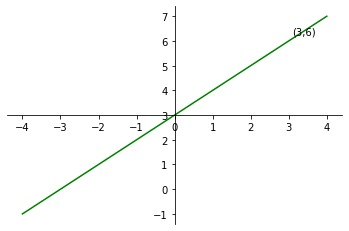
\includegraphics[width=7cm,height = 7cm]{Assignment_2.png}
    
    \label{regeq}
\end{figure}
 
\end{document}
